\section{Performance Discussion} \label{sect:experimental}

\begin{figure*}[t]
  \centering
  \subfigure[\small One Process failing at a time]{
    \label{fig:onebyone}
    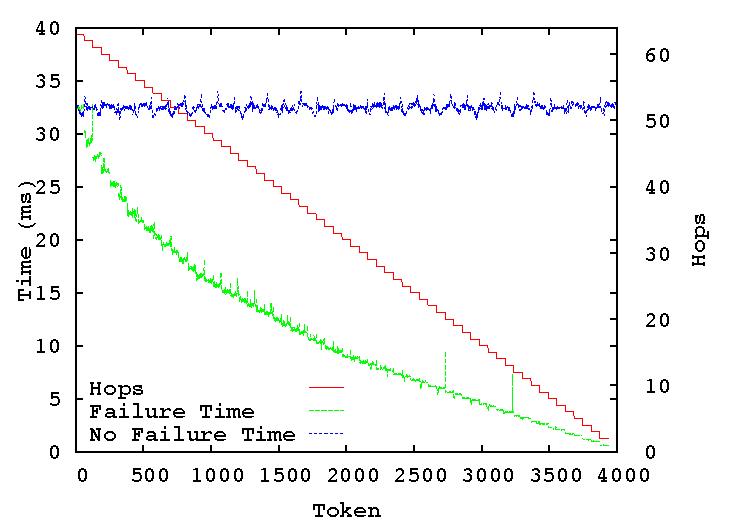
\includegraphics[scale=0.65]{figures/even.pdf}
  }
  \subfigure[\small Two concurrently failing processes]{
    \label{fig:burst}
    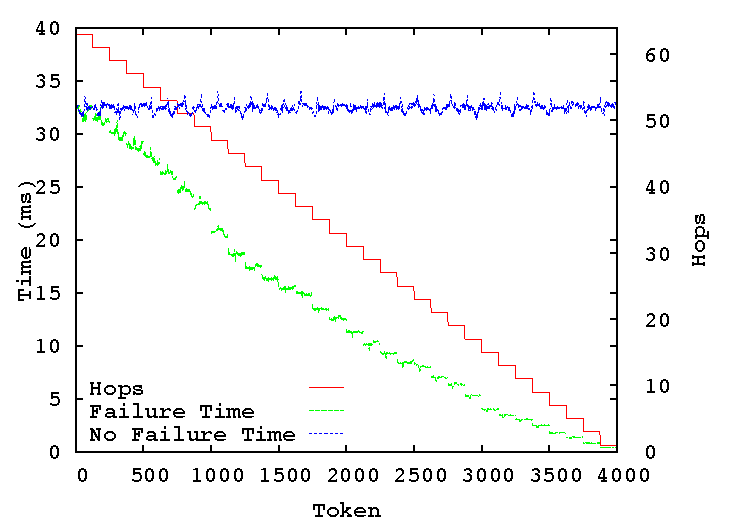
\includegraphics[scale=0.65]{figures/burst.pdf}
  }
  \caption{Token Roundtrip Time with Evenly Failing Processes}
  \label{fig:even}
\end{figure*}

%\begin{figure*}[t]
%  \centering
%  \subfigure[\small N/2 Processes Failing at Midpoint]{
%    \label{fig:major}
%    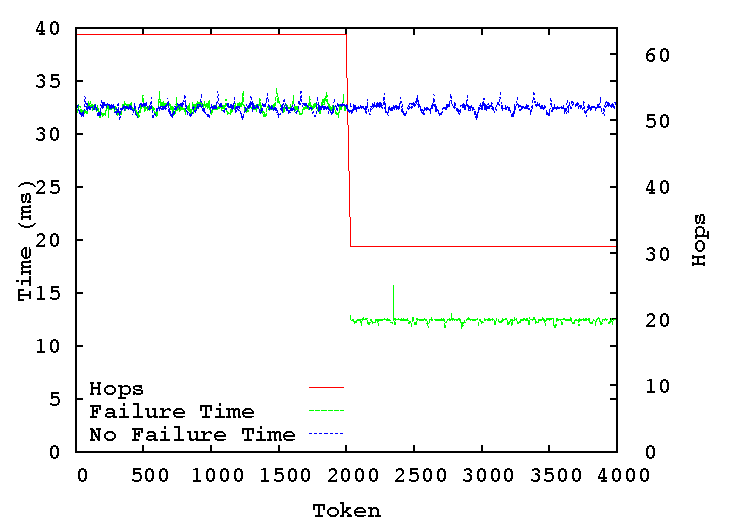
\includegraphics[scale=0.50]{major.pdf}
%  }
%  \subfigure[\small N-2 Processes Failing at Midpoint]{
%    \label{fig:critical}
%    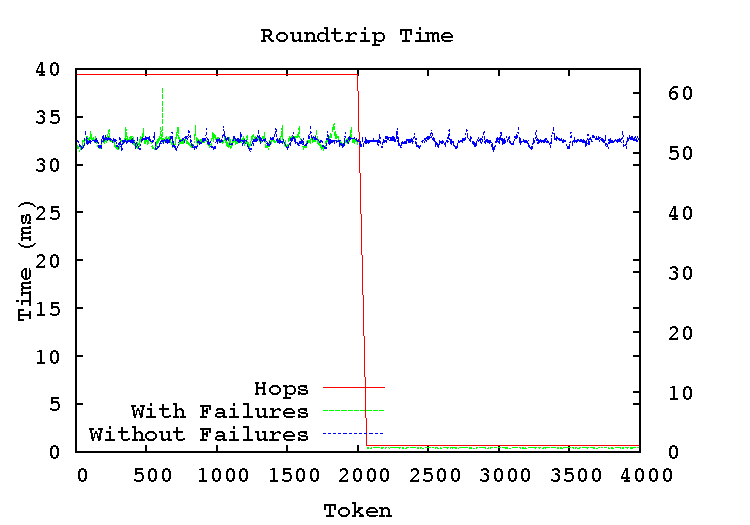
\includegraphics[scale=0.50]{critical.pdf}
%  }
%  \caption{Token Roundtrip Time with Many Simultaneous Failing Processes}
%  \label{fig:many}
%\end{figure*}

\begin{figure*}[t]
  \centering
  \subfigure[\small Detection Time for Failures]{
    \label{fig:detection}
    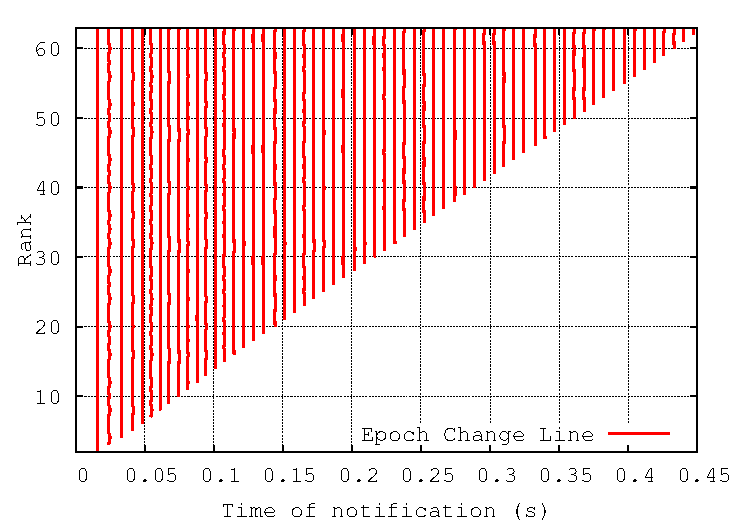
\includegraphics[scale=0.65]{figures/epochs-lines.pdf}
  }
  \subfigure[\small Overhead Introduced by Changes]{
    \label{fig:overhead}
    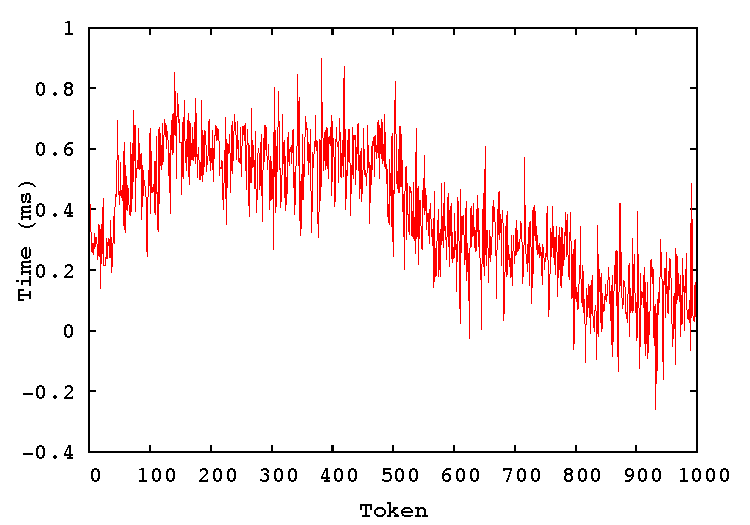
\includegraphics[scale=0.65]{figures/overhead.pdf}
  }
  \caption{Overheads of the Resilient Runtime}
  \label{fig:overheads}
\end{figure*}

% -- Runtime --
In this section we describe the results of our work to this point. First we present a model
to describe the expected results of our resilient runtime's failure notification
method. Second, we will demonstrate the observed values derived from our tests
performed on a 64 node cluster within Grid5000. \footnote{Experiments presented
in this paper were carried out using the Grid'5000 experimental testbed, being
developed under the INRIA ALADDIN development action with support from CNRS,
RENATER and several Universities as well as other funding bodies (see
https://www.grid5000.fr)}

\subsection{Performance Model} \label{subsect:performance_model}
% Describe the model that our runtime is expected to fit within.

We devised a model of the expected failure detection behavior of our runtime
system. Let $T$ be the initial routing topology of the system. Let $L_T(d, f,
H)$ be the time it takes process $d$ to notice a failure of process $f$, knowing
that $\forall q\in H$, $q$ is also failed (potentially before $f$). We call
$L_T(d, f, H)$ the latency of detection of $d$ for $f$ knowing $H$.

$$L_T(d, f, H) \leq \alpha_0 + \gamma D_{T \backslash H \cup \{f\}}(f, d)$$

Where $\alpha_0$ is the time taken by an immediate neighbor of $f$ to detect its
failure, $\gamma$ is the point-to-point message latency, and $D_{T \backslash H
\cup \{f\}}(f, d)$ is the distance (in number of hops) between $f$ and $d$ in
the routing topology, $T \backslash H\bigcup \{f\}$. Note that this distance
could shrink as processes between $f$ and $d$ in the routing topology fail.

Whatever the history of failures $H$, if $|T| = n$, then $D_{T \backslash H}(s,
d) \leq \log_2(n)$. This is true because the routing layer we use is a binomial
tree, which has a maximum depth of $log_2(n)$. Also, when repairing the routing
tree after a failure, the routing layer does not add new hops, it only mends the
routes by removing failed processes from the topology and creating links between
the next surviving neighbors both above and below $f$. Thus, for system $Bin(n)$
with $n$ processes initially, with a fault tolerant binomial tree routing layer,

$$\forall d, f\in Bin(n), \forall H \subseteq Bin(n),$$
$$L_{Bin(n)}(d, f, H) \leq \alpha_0 + \gamma \log_2(n)$$

This shows that our improved routing topology should perform no worse than a
fault free one following a process failure.

\subsection{Performance Data} \label{subsect:performance_data}

% Ring test with binomial routing
% Emphasize "Proof of Concept" rather than large scale performance runs

When validating the runtime work described in Section~\ref{sect:runtime}, our
goal was to devise a test that would confirm its correctness while being simple
to describe and understand. It should be emphasized that this is not necessarily
representative of a specific application, but it does demonstrate that the
improved runtime would be able to support a full application in the presence of
a process failure. It is designed to show that the runtime can heal its routing
layers following multiple and catastrophic process failures. Once a resilient
MPI layer is built on top of the runtime, a full application could be tested
with MPI semantics.

Our test is a ring test which dispatches multiple tokens from process 0. These
tokens are passed around the ring in increasing sequential order until they
reach process 0 again where various measurements are made. This is a simplistic
test and therefore not designed to demonstrate the recovery of a lost token,
however the test could easily be modified to demonstrate that behavior as
described by Hursey~\cite{Hursey:vb}. Process 0 generates 4000 tokens and passes
them along. As the tokens are passed around the ring, the test generates
failures at predetermined times to give an idea of the behavior of the runtime
with different failure patterns. The loss of tokens gives an idea of how long
the routing layer took to patch itself and continue sending tokens to the next
living process.

% Describe the graphs

Figure~\ref{fig:even} shows the round trip time of each of the tokens as the
failures are generated within the system. Each graph shows both the time from a
failure free run and a run with a specific failure pattern. The graphs also
show how many hops each token traversed while traveling around.

% Compare ring/token test FF vs. failure

In Figure~\ref{fig:onebyone}, processes fail one at a time in evenly spaced
intervals until only 2 processes remain. As each process fails, the round trip
time decreases linearly. This is the expected behavior as each token must
traverse fewer processes until it reaches process 0 again. The number of hops
decreases slowly as each process fails, but the round trip time with failures
actually decreases at a greater rate temporarily. This is because the buffers at
the first few processes become full at the beginning of the run when the tokens
are still being generated. As the buffers clear the first few processes, the
round trip time stabilizes.% into a linear speedup.

In Figure~\ref{fig:burst}, processes fail in groups of two. This shows that the
runtime can withstand larger groups of processes failing at roughly the same
time.
% This would simulate a two processor node failing at once.
 The gaps in the
graph show the points at which some tokens are lost. This is expected as the
application makes no attempt to recover or regenerate tokens temporarily hosted
by failed processes, and simply continues to run with whatever tokens return
back to the originating process.

%% Kill 1/2 in middle
%Figure~\ref{fig:major} introduces much larger failures at a time. In this test,
%half of the processes fail all at once at the midpoint of the run. While it
%takes the runtime some time to discover all of the failures, as illustrated by
%the larger number of lost tokens, it does eventually recover from the losses and
%any tokens that were not on one of the failed processes at the time of the
%failure continue around the ring until process 0 receives them again.
%
%% Kill p - 2 in middle
%Figure~\ref{fig:critical} introduces a critical failure. In this test, all but
%two processes are killed at the same time at the midpoint of the run. Again, the
%runtime requires a discovery period before stabilizing, but it is able to
%recover and continue delivering the remaining tokens back to process 0.
%Figures~\ref{fig:major} and~\ref{fig:critical} are encouraging as they show that
%the runtime can withstand any number of failures at any time. This
%implementation can withstand concurrent or consecutive failures without
%requiring any minimal ``cooling off'' period between failures.

Our runtime is also able to handle failure rates much higher than one or two
processes at a time. In other tests, we were able to handle rates of $n/2$ or
$n-2$ simultaneous failures. This is encouraging as it shows that the runtime
can withstand any number of failures at any time. The failures can occur
concurrently or consecutively without requiring a ``cooling off'' period between
failures.

% Detection Time
Figure~\ref{fig:detection} shows the detection and notification time for each
failure. It uses the same case as figure~\ref{fig:onebyone} where failures occur
evenly throughout the lifetime of the application. Each line represents the
detection time of each epoch among all the processes, collected using the ad-hoc
fault handler. 
% To reduce the effect of clock drift, the time is measured from
% the beginning of the local application rather than attempting to synchronize
% with a single value from process 0. 
When the line is straight, it
demonstrates that the latency of detection and notification is
relatively low among all the remaining process. This figure shows that the
detection time for the all processes is very tight, demonstrating that all
processes can maintain a consistent view of the current epoch. The earlier
epochs have a slightly varying detection time as the notification messages have
further to travel through the routing layer, but as the tree becomes smaller as
it is repaired, the oscillations decrease, demonstrating a much smaller window
of time for each epoch.

% Overhead
Figure~\ref{fig:overhead} shows the overhead that was introduced by modifying
the \ompi source code. It compares the runtime of a fault-free case using both
our implementation of the \ompi runtime, and the revision 24614 of the \ompi
trunk. The overhead was measured on a local 8 node development cluster with
minimal system noise to eliminate outside effects on the data. We subtract the
round trip time for each token in the resilient version of \ompi from the same
test using the trunk version of \ompi. The results show that the changes made to
the code actually had little impact on performance in the fault-free case.
Variations can be explained by the network jitter and the small increase in the
header size of the messages due to the epoch algorithm.

